\documentclass[]{ximera}
%handout:  for handout version with no solutions or instructor notes
%handout,instructornotes:  for instructor version with just problems and notes, no solutions
%noinstructornotes:  shows only problem and solutions

%% handout
%% space
%% newpage
%% numbers
%% nooutcomes

%I added the commands here so that I would't have to keep looking them up
%\newcommand{\RR}{\mathbb R}
%\renewcommand{\d}{\,d}
%\newcommand{\dd}[2][]{\frac{d #1}{d #2}}
%\renewcommand{\l}{\ell}
%\newcommand{\ddx}{\frac{d}{dx}}
%\everymath{\displaystyle}
%\newcommand{\dfn}{\textbf}
%\newcommand{\eval}[1]{\bigg[ #1 \bigg]}

%\begin{image}
%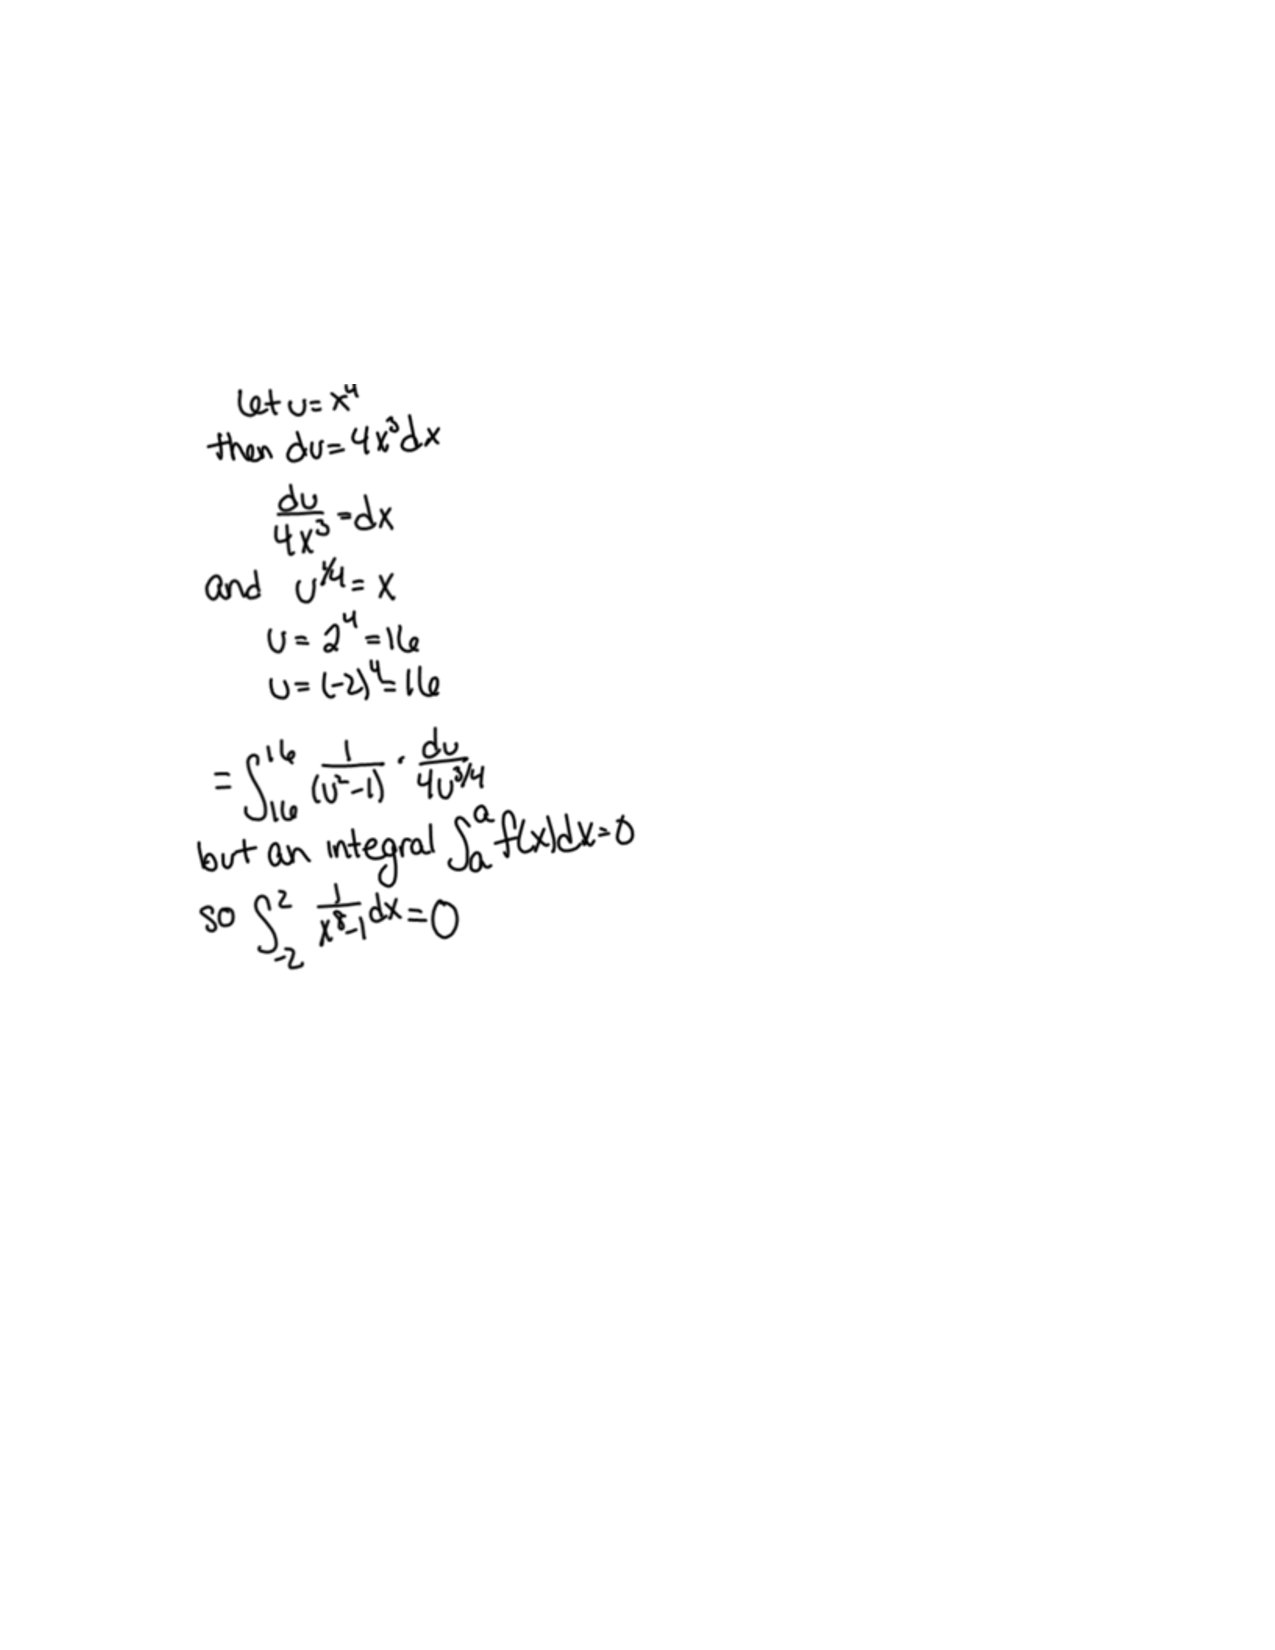
\includegraphics[trim= 170 420 250 180]{Figure1.pdf}
%\end{image}

%add a ``.'' below when used in a specific directory.
\newcommand{\RR}{\mathbb R}
\renewcommand{\d}{\,d}
\newcommand{\dd}[2][]{\frac{d #1}{d #2}}
\renewcommand{\l}{\ell}
\newcommand{\ddx}{\frac{d}{dx}}
\newcommand{\dfn}{\textbf}
\newcommand{\eval}[1]{\bigg[ #1 \bigg]}

\usepackage{multicol}

\renewenvironment{freeResponse}{
\ifhandout\setbox0\vbox\bgroup\else
\begin{trivlist}\item[\hskip \labelsep\bfseries Solution:\hspace{2ex}]
\fi}
{\ifhandout\egroup\else
\end{trivlist}
\fi} %% we can turn off input when making a master document

\title{Vectors in three dimensions}  

\begin{document}
\begin{abstract}		\end{abstract}
\maketitle



\begin{comment}
\section{Warm up:}

	\begin{freeResponse}
	
	\end{freeResponse}
	
\begin{instructorNotes}

\end{instructorNotes}
\end{comment}







\section{Group work:}



%problem 1
\begin{problem}
Solve the following problems:
	\begin{enumerate}
	\item  Which of the points $(6,2,3)$, $(-5,-1,4)$, and $(0,3,8)$ is closest to the $xz$-plane?  
	Which point lies on the $yz$-plane?
	
	\item  Write an equation of the circle of radius $2$ centered at $(-3,4,1)$ that lies in a plane parallel to the $xy$-plane.
	
	\item  Describe the sphere $x^2 + y^2 + z^2 + 6x - 14y - 2z = 5$ (ie, find its center and radius).
	
	\item  Find a vector whose magnitude is $311$ and is in the same direction as the vector $\langle 3,-6,7 \rangle$.
	\end{enumerate}
	
	\begin{freeResponse}
	\begin{enumerate}
	\item  The $xz$-plane has equation $y=0$.  
	The distance from a point $(a,b,c)$ to $y=0$ is just $|b|$.  
	So
		\begin{align*}
		&(6,2,3) \text{ has distance }2  \\
		&(-5,-1,4) \text{ has distance }1  \\
		&(0,3,8) \text{ has distance }3
		\end{align*}
	Therefore, the point $(-5,-1,4)$ is closest to the $xz$-plane.  
	
	The $yz$-plane is $x=0$, and so the point $(0,3,8)$ is on the $yz$-plane.
	
	
	
	\item  A plane parallel to the $xy$-plane has equation $z = \#$.  
	We are looking for such a plane containing the point $(-3,4,1)$, and so the plane is $z=1$.  
	Therefore, the equation is
		\[
		\boxed{ (x+3)^2 + (y-4)^2 = 4 \;, \; z = 1.   }
		\]
		
		
	
	\item  We complete the square with respect to all three variables.
		\begin{align*}
		x^2 + y^2 + z^2 + 6x - 14y - 2z &= 5  \\
		(x^2 + 6y + 9) + (y^2 - 14y + 49) + (z^2 - 2z + 1) &= 5 + 9 + 49 + 1  \\
		(x+3)^2 + (y-7)^2 + (z-1)^2 &= 64.
		\end{align*}
	So, the center of the sphere is $(-3,7,1)$ and its radius is $8$.
	
	
	
	\item  Let $\vec{v} = \langle 3,-6,7 \rangle$.  
	Then
		\begin{align*}
		| \vec{v} | &= \sqrt{3^2 + (-6)^2 + 7^2}  \\
		&= \sqrt{9 + 36 + 49}  \\
		&= \sqrt{94}.
		\end{align*}
	So a unit vector in the same direction as $\vec{v}$ is
		\[
		\frac{1}{\sqrt{94}} \langle 3,-6,7 \rangle
		\]
	and therefore a vector with magnitude $311$ in the same direction as $v$ is
		\[
		\boxed{\frac{311}{\sqrt{94}} \langle 3,-6,7 \rangle}
		\]
	
	\end{enumerate}
	\end{freeResponse}
	
\end{problem}

\begin{instructorNotes}

\end{instructorNotes}







%problem 2
\begin{problem}
A $500kg$ lead hangs from three cables of equal length that are located at the points $(-2,0,0)$, $(1, \sqrt{3},0)$, and $(1, -\sqrt{3},0)$.  
The load is located at $(0,0,-2 \sqrt{3})$.  
Find the vectors describing the forces on the cables due to the load.
	\begin{freeResponse}
	Let $A = (1,-\sqrt{3},0)$, $B = (1, \sqrt{3},0)$, and $C = (-2,0,0)$, and let $M = (0,0, -2\sqrt{3})$.  
	Let $\vec{a}$, $\vec{b}$, and $\vec{c}$ denote the vectors from $A$, $B$, and $C$ to $M$, respectively.  
	ie, 
		\begin{align*}
		&\vec{a} = \langle 0-1, 0 - (-\sqrt{3}), -2 \sqrt{3}-0 \rangle = \langle -1, \sqrt{3}, -2 \sqrt{3} \rangle  \\
		&\vec{b} = \langle 0-1, 0 - \sqrt{3}, -2 \sqrt{3} - 0 \rangle = \langle -1, -\sqrt{3}, -2 \sqrt{3} \rangle  \\
		&\vec{c} = \langle 0- (-2), 0 - 0, -2 \sqrt{3} - 0 \rangle = \langle 2, 0, -2 \sqrt{3} \rangle .
		\end{align*}
		
		%\begin{image}
		%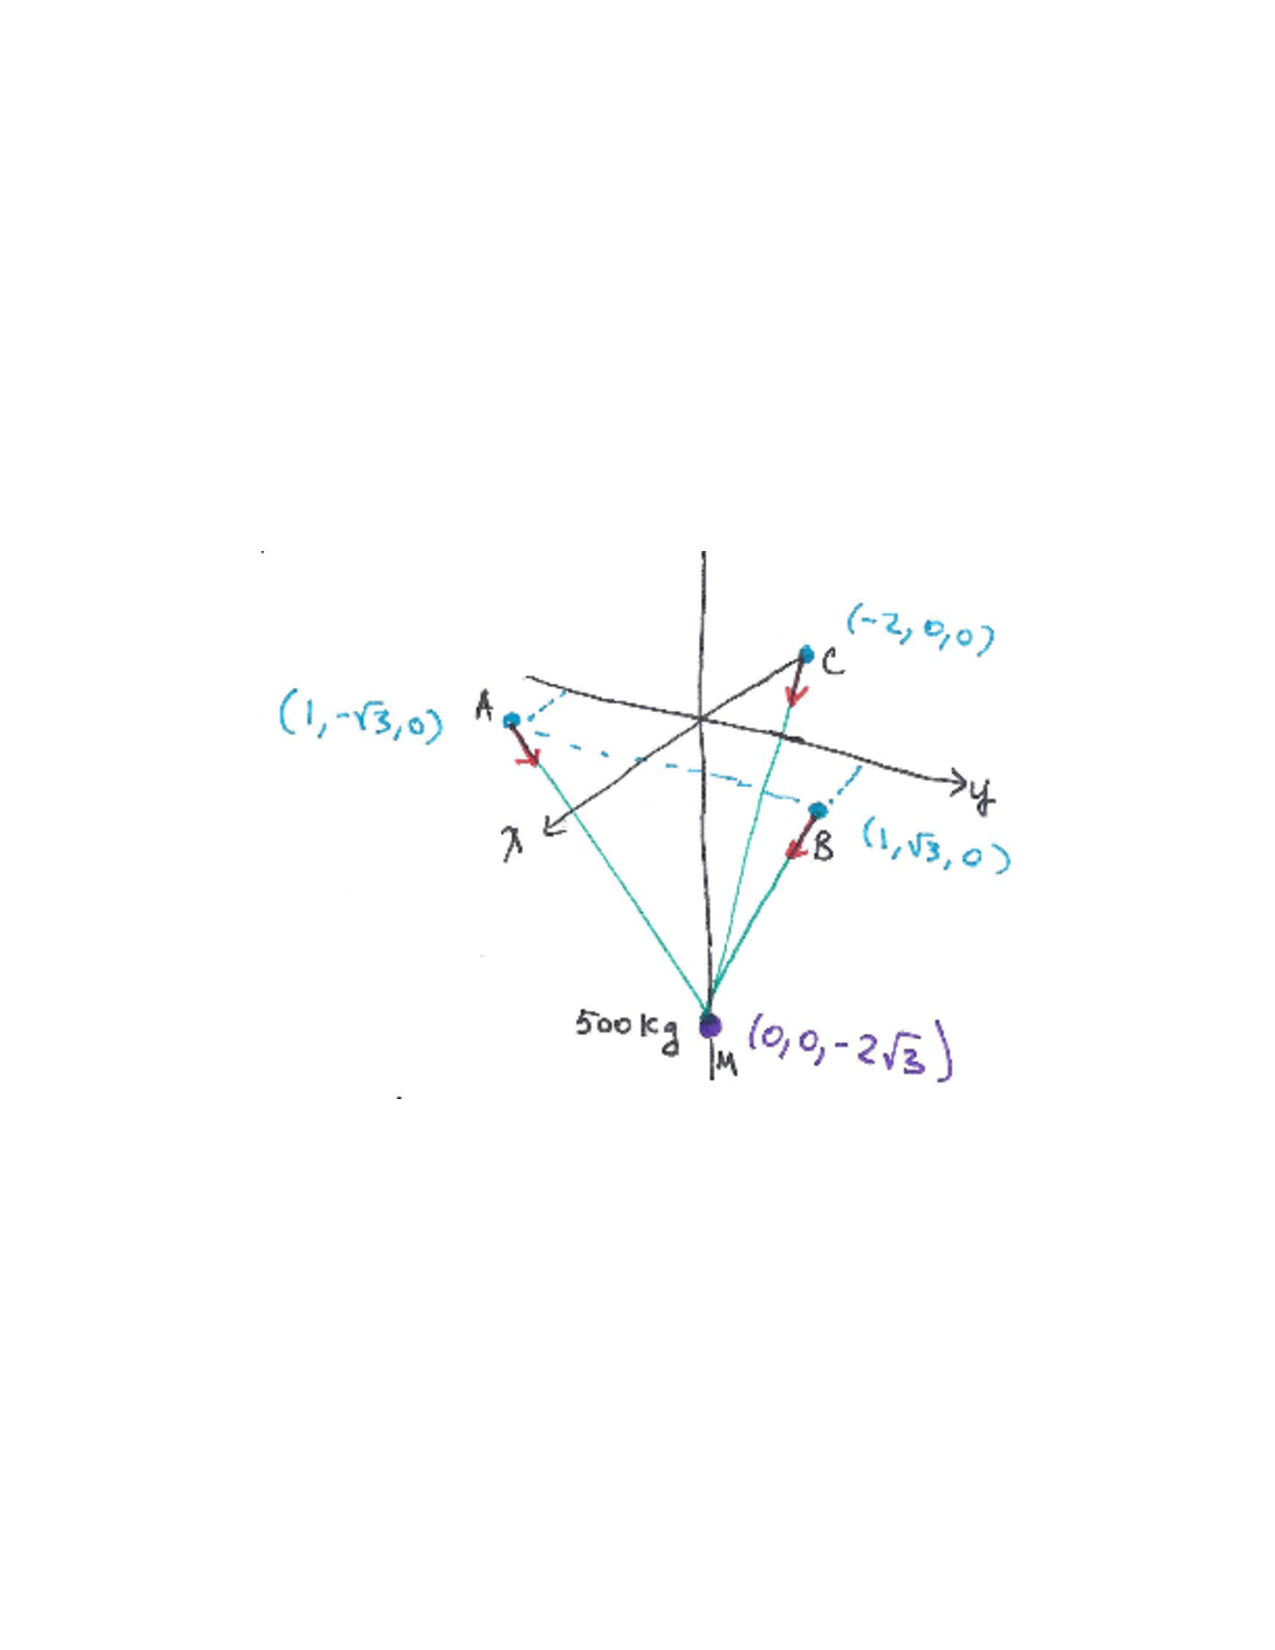
\includegraphics[trim= 170 420 250 180]{Figure12-2-1.pdf}
		%\end{image}
		
	Notice that
		\[
		\| \vec{a} \| = \| \vec{b} \| = \| \vec{c} \| = 4
		\]
	and so unit vectors in the directions of $\vec{a}$, $\vec{b}$, and $\vec{c}$ are
		\begin{align*}
		&\vec{u}_a = \frac{1}{4} \langle -1, \sqrt{3}, -2\sqrt{3} \rangle  \\
		&\vec{u}_b = \frac{1}{4} \langle -1, - \sqrt{3}, -2\sqrt{3} \rangle  \\
		&\vec{u}_c = \frac{1}{4} \langle 2, 0, -2\sqrt{3} \rangle  .
		\end{align*}
		
	The force on $M$ due to gravity is 
		\[
		\langle 0,0, -500 g \rangle
		\]
	where $g$ is the gravitational constant.  
	We need to find real numbers $x$, $y$, and $z$ such that
		\begin{align}
		&-\frac{1}{4} x - \frac{1}{4} y + \frac{1}{2} z = 0    \qquad \Longrightarrow \qquad x+y-2z=0  \label{eqn1}  \\
		&\frac{\sqrt{3}}{4} x - \frac{\sqrt{3}}{4} y + 0z = 0  \qquad \Longrightarrow \qquad x-y=0  \label{eqn2}  \\
		&- \frac{\sqrt{3}}{2} x - \frac{\sqrt{3}}{2} y - \frac{\sqrt{3}}{2} z = -500g  \quad \Longrightarrow \quad x+y+z= \frac{1000g}{\sqrt{3}}. \label{eqn3}
		\end{align}
	By equation \eqref{eqn2} we have that $x=y$.  
	Substituting this into equation \eqref{eqn1} we also see that $x=z$.  
	So $x=y=z$.  
	We plug this into equation \eqref{eqn3} to get that
		\[
		3x = \frac{1000g}{\sqrt{3}} \qquad \Longrightarrow \qquad x = \frac{1000g}{3\sqrt{3}}.
		\]
		
	Thus,
		\begin{itemize}
		\item  The force along $AM$ is $\boxed{\frac{1000g}{3\sqrt{3}} \cdot \frac{1}{4} \langle -1, \sqrt{3},-2\sqrt{3} \rangle}$.
		\item  The force along $BM$ is $\boxed{\frac{1000g}{3\sqrt{3}} \cdot \frac{1}{4} \langle -1, -\sqrt{3}, -2\sqrt{3} \rangle}$.
		\item  The force along $CM$ is $\boxed{\frac{1000g}{3\sqrt{3}} \cdot \frac{1}{4} \langle 2,0,-2\sqrt{3} \rangle }$.
		\end{itemize}
	\end{freeResponse}
		
\end{problem}

\begin{instructorNotes}
Students need to take into account that the mass, and not the force, is given.  
The students should also take advantage of the fact that the vectors are all of the same magnitude.  
\end{instructorNotes}







\begin{comment}
%problem 3
\begin{problem}

	\begin{freeResponse}
	
	\end{freeResponse}

\end{problem}

\begin{instructorNotes}

\end{instructorNotes}
\end{comment}
















	
	
	
	
	
	
	
	
	

	










								
				
				
	














\end{document} 


















